% ICCIT 2026 camera-ready version (6-page limit, including references).
% The full-length version with all tables, figures, and supporting analyses is main.tex
% (extended technical report); every number below also appears there and is checked by
% step4 dataset/verify_claims.py against the committed per-row outputs.
\documentclass[conference]{IEEEtran}
\IEEEoverridecommandlockouts
\usepackage{cite}
\usepackage{amsmath,amssymb,amsfonts}
\usepackage{booktabs}
\usepackage{graphicx}
\usepackage{array}
\usepackage{makecell}
\usepackage{url}
\usepackage{tikz}
\usepackage{pgfplots}
\pgfplotsset{compat=1.17}

\begin{document}

\title{Attributing Security in a Local, Zero-Cost Defense-in-Depth Pipeline for Retrieval-Augmented Generation}

% TODO camera-ready: replace with the authors' names, affiliations, and e-mails.
\author{\IEEEauthorblockN{Anonymous Authors}}

\maketitle

\begin{abstract}
Retrieval-Augmented Generation (RAG) lets an attacker place instructions or false facts in the context window through retrieved passages. Deployed systems stack imperfect defenses but rarely measure which layer provides the protection. We build a thirteen-stage, fully local, zero-cost defense pipeline and attribute its security stage by stage on 920 evaluation rows across seven sets, including independent PoisonedRAG, BIPIA, and deepset data, with paired exact tests. Attack success on 200 planted attacks falls from 29.5\% undefended to 3.5\% ($p<10^{-13}$), and a fresh rerun reproduces this (29.0\% to 3.0\%). On the same attacks the pipeline outperforms an LLM-Guard firewall (21.0\%) and Spotlighting (23.0\%) ($p<10^{-7}$) and matches ControlNET (4.5\%, $p=0.77$) with somewhat better benign utility. Ablation shows that three layers (per-chunk sanitization, grounding, and refusal on detection) are statistically indistinguishable from the seven-layer stack, with the gap bounded at 2.4 points at $n=424$. A co-activation detector for conjunctive sub-threshold attacks cannot fire validly on saturated classifier scores, for a structural reason we prove; graded logit margins partly repair it. Knowledge corruption is out of reach: on PoisonedRAG the defended pipeline is no better than undefended RAG (90.7\% vs.\ 91.3\%, $p=1.0$).
\end{abstract}

\begin{IEEEkeywords}
Retrieval-augmented generation, prompt injection, LLM security, defense in depth, local inference.
\end{IEEEkeywords}

\section{Introduction}
RAG conditions a language model on passages retrieved at query time~\cite{lewis2020rag}, so every retrieved passage is an untrusted input channel. An attacker who can edit retrievable content can deliver instructions (indirect prompt injection~\cite{greshake2023}, ranked first in the OWASP Top~10 for LLM applications~\cite{owasp2025}) or false facts (knowledge corruption~\cite{zou2025poisonedrag}) without the user's involvement. Most defenses rely on paid cloud services, which expose the data a private deployment is meant to protect. We therefore require every component to run locally, under an open licence, at no API cost.

Real deployments stack several imperfect layers, and when such a pipeline stops an attack it is rarely clear which layer was responsible. This paper addresses that attribution question. Our contributions are: (C1) an attribution protocol that runs every configuration on identical rows, scores each row by a machine-checkable outcome, and tests each stage with leave-one-out, add-one-in, and subset ablations under exact paired tests; (C2) a comparison with existing defenses on the same rows; (C3) a negative result, with a closed-form argument, for co-activation detection on saturated classifier scores, and a graded-margin repair; and (C4) a measured scope boundary: the defense does not extend to signature-free knowledge corruption. We do not claim a new detector; the components are known, and the contribution is measuring which of them carry the security.

\section{Related Work}
Adaptive RAG systems such as Self-RAG~\cite{asai2024selfrag}, CRAG~\cite{yan2024crag}, and FLARE~\cite{jiang2023flare} revise retrieval with late signals; our closed-loop controller adopts this structure for security risk. Prompt injection was shown by Perez and Ribeiro~\cite{perez2022}, extended to retrieved content by Greshake et al.~\cite{greshake2023}, and formalized by Liu et al.~\cite{liu2024formalizing}. Detectors include a fine-tuned DeBERTa-v3 injection classifier~\cite{he2021debertav3,protectai2024} and Llama Guard~\cite{inan2023llamaguard}; structural defenses include Spotlighting~\cite{hines2024spotlighting}, the dual-LLM pattern~\cite{willison2023dual}, and CaMeL~\cite{debenedetti2025camel}; grounding checks follow RAGAS~\cite{es2023ragas}. Closest to our setting are ControlNET~\cite{yao2025controlnet}, which detects malicious queries from activation shifts, the Sentinel--Strategist orchestrator (ADO)~\cite{palleria2026ado}, and the layered framework of Saleem et al.~\cite{saleem2026layered}, which evaluates all subsets of its three layers. These works report point estimates without confidence intervals or paired tests, and none reports a component of its own system that fails to contribute (Table~\ref{tab:positioning}).

\begin{table}[t]
\centering
\caption{Positioning against related RAG and prompt-injection defenses. \checkmark{} = provided; -- = not reported.}
\label{tab:positioning}
\setlength{\tabcolsep}{2.6pt}
\begin{tabular}{lccccc}
\toprule
Work & \makecell{Fully\\local} & \makecell{Context\\defense} & \makecell{Stage-level\\attribution} & \makecell{Paired\\tests} & \makecell{Negative\\results} \\
\midrule
Spotlighting~\cite{hines2024spotlighting} & -- & \checkmark & -- & -- & -- \\
CaMeL~\cite{debenedetti2025camel} & -- & \checkmark & -- & -- & -- \\
ControlNET~\cite{yao2025controlnet} & \checkmark & \checkmark & -- & -- & -- \\
ADO~\cite{palleria2026ado} & \checkmark & \checkmark & -- & -- & -- \\
Layered~\cite{saleem2026layered} & partial$^a$ & \checkmark & subsets$^b$ & -- & -- \\
\textbf{This work} & \checkmark & \checkmark & \checkmark & \checkmark & \checkmark \\
\bottomrule
\multicolumn{6}{l}{\footnotesize $^a$GPT-4o target and judge via API; others local.} \\
\multicolumn{6}{l}{\footnotesize $^b$All seven layer subsets; point estimates, no tests or CIs.} \\
\end{tabular}
\end{table}

\section{Method}\label{sec:method}
The pipeline wraps a RAG core in a thirteen-stage cascade. Stage~2 normalizes the prompt (NFKC, \texttt{ftfy}, decoding). The input gate (Stage~3) fuses the DeBERTa-v3 injection score with a Llama Guard~3 verdict into a risk score $r$ and a decision (allow, review, block). The same $r$ is propagated forward and tightens the downstream stages for that request. After embedding (bge-m3) and FAISS retrieval (Stages~4--5), Stage~6 scans each retrieved chunk for embedded instructions, redacts flagged chunks (threshold 0.50, tightened to 0.30 when $r>0.45$), and inserts a canary token. Stage~7 reranks with a cross-encoder; Stage~8 builds a prompt that treats the context as data; Stage~9 generates with three local models (Llama~3.2, Mistral~7B, Qwen2.5), whose disagreement is a risk signal; Stage~10 checks grounding and the canary; Stages~11--12 mask PII (Presidio) and apply DLP; Stage~13 returns the answer or a refusal (Table~\ref{tab:stages}).

\begin{table}[t]
\centering
\caption{The cascade. Every model runs locally.}
\label{tab:stages}
\footnotesize
\setlength{\tabcolsep}{2pt}
\resizebox{\columnwidth}{!}{%
\begin{tabular}{lll}
\toprule
Stage & Function & Local tool \\
\midrule
2 & Normalization & \texttt{ftfy}, NFKC \\
3 & Fusion input gate & DeBERTa-v3, Llama Guard 3 \\
4--5 & Embedding, search & bge-m3, FAISS \\
6 & Per-chunk sanitization, canary & LLM-Guard scanner \\
7 & Reranking & bge-reranker-v2-m3 \\
8 & Data-only prompt & LangChain LCEL \\
9 & Generator ensemble & Llama 3.2, Mistral, Qwen2.5 \\
10 & Grounding, canary check & Lexical + cross-encoder \\
10A/B & Co-activation; controller & Noisy-OR; retry/refuse \\
11--12 & PII masking, DLP & Presidio, regex/Luhn \\
13 & Safe response & Refusal, audit log \\
\bottomrule
\end{tabular}}
\end{table}

\textbf{Extension A: multi-vector risk fusion.} For conjunctive attacks that split an instruction between the query and a chunk, a query channel $x_q=\max(s_{\mathrm{inj}}, r)$ and a context channel $x_c=\max_j s_{\mathrm{inj}}(d_j)$ are fused by the noisy-OR $R=1-(1-x_q)(1-x_c)$; the detector fires if both channels exceed their floors ($f_q=0.228$, $f_c=0.30$) and $R\ge0.542$. A fire is \emph{valid} only if both channels also stay below their block thresholds.
\textbf{Extension B: closed-loop controller.} Using late signals (disagreement, grounding, canary, co-activation), it accepts, re-verifies, retries with broader retrieval, or refuses; it is fail-closed.

\section{Experimental Setup}\label{sec:setup}
The knowledge base is rag-mini-wikipedia~\cite{ragmini2024} (3{,}200 passages); gate thresholds were set on public injection, jailbreak, and toxicity data. Table~\ref{tab:evalsets} lists the seven evaluation sets. \emph{Protocol~A} is a stratified 220-row slice whose classes each isolate one threat model and whose rows carry machine-checkable expectations (gate decision, redaction, canary); it runs the complete pipeline. \emph{Protocol~B} scores what the user receives: each of 200 attack rows plants a false fact in a retrieved chunk and nudges the query toward it, and the attack succeeds if the response contains the planted target and not the true answer; 200 benign questions measure refusals and correctness. Protocol~B uses the same stage implementations through a harness that toggles seven layers independently with a single generator (\texttt{llama3.2:3b}, temperature 0.2, seed 42), so arms differ only in the toggled layer. Three external sets were not built by us: PoisonedRAG~\cite{zou2025poisonedrag}, BIPIA~\cite{yi2023bipia}, and deepset prompt-injections~\cite{deepset2023pi}. All runs used one laptop (Table~\ref{tab:env}); the LLMs are served by Ollama on the GPU and the encoders run on the CPU. Gate thresholds are $\tau_{\text{review}}=0.35$ and $\tau_{\text{block}}=0.60$; retrieval uses $k=5$ and rerank top-3.

\begin{table}[t]
\centering
\caption{Hardware, software, and models used in all experiments.}
\label{tab:env}
\setlength{\tabcolsep}{3pt}
\small
\begin{tabular}{p{2.3cm}p{5.6cm}}
\toprule
Component & Specification \\
\midrule
CPU / RAM & AMD Ryzen 5 7640HS (6C/12T), 16\,GB (15.2\,GB usable) \\
GPU & NVIDIA GeForce RTX 4060 Laptop, 8\,GB VRAM, driver 566.24 \\
OS / runtime & Windows 11 Home (26200), Python 3.11.9, Ollama 0.40.16 \\
Libraries & PyTorch 2.12.0 (CPU build; CUDA 12.6 build for the GPU-encoder test), Transformers 4.51.3, sentence-transformers 5.5.1, llm-guard 0.3.16, Presidio 2.2.358, FAISS-cpu 1.14.2 (IndexFlatIP), spaCy 3.8.14, ftfy 6.3.1, langchain-ollama 1.1.0, SciPy 1.17.1 \\
Input gate & protectai/deberta-v3-base-prompt-injection-v2 (ONNX, CPU); \texttt{llama-guard3:1b} (Q8\_0) \\
Retrieval & BAAI/bge-m3 (embedding); BAAI/bge-reranker-v2-m3 (rerank, judge) \\
Generators & \texttt{llama3.2:3b}, \texttt{mistral:7b}, \texttt{qwen2.5:3b} (Q4\_K\_M) \\
\bottomrule
\end{tabular}
\end{table}

\textbf{Statistics.} Every configuration is applied to the same rows, so comparisons use the exact two-sided McNemar test on discordant rows~\cite{mcnemar1947}, reported with the discordant counts; proportions carry 95\% Wilson intervals~\cite{wilson1927}. A large $p$ means no detectable difference at that $n$, not equivalence. Leave-one-out and subset families use Bonferroni correction.

\begin{table}[t]
\centering
\caption{Evaluation sets (920 rows).}
\label{tab:evalsets}
\footnotesize
\setlength{\tabcolsep}{2pt}
\begin{tabular}{lrll}
\toprule
Set & $n$ & Source & Outcome scored \\
\midrule
Adversarial slice (A) & 220 & Constructed & Gate, redaction, canary \\
Planted attacks (B) & 200 & Constructed & Target in response \\
Benign questions (B) & 200 & rag-mini-wiki & Refusal, correctness \\
Semantic free-text (B) & 40 & Constructed & Target in response \\
PoisonedRAG & 150 & External & Target in response \\
BIPIA & 50 & External & Block, manual reading \\
deepset & 60 & External & Gate decision \\
\bottomrule
\end{tabular}
\end{table}

\section{Results}\label{sec:results}
\subsection{Protocol A: Specificity, Indirect Injection, Canaries}
The gate flags none of the 80 benign rows (0/80, [0, 4.6]\%); downstream, 10 benign rows are refused (14 without the controller). All 40 poisoned chunks are redacted at Stage~6, and every poisoned chunk across classes (74/74) is removed before generation. No canary leaks into any of the 132 delivered answers; the canary was checked on the 175 rows that reached Stage~10, and the other 45 were blocked earlier, 44 at the gate. The gate flags 29--30 of 40 direct injections (25 blocked); the cascade blocks all 40 once the propagated risk tightens the downstream stages. The controller adds no measured security over the single-pass pipeline, but refuses fewer rows (88 vs.\ 101 blocked; 70 vs.\ 66 benign answers delivered). Canary integrity is a proxy, so we score output behavior directly in Protocol~B.

\subsection{Ablation: Which Layers Carry the Defense?}\label{sec:ablation}
Table~\ref{tab:ablation} toggles the seven layers on the 200 planted attacks. No single layer approaches the full stack: the best (grounding, sanitization, refusal) leave 15--18\% ASR, and the guarded prompt alone \emph{raises} ASR to 53.0\%. The layers are complementary, and the three-layer subset sanitize+ground+refuse is statistically indistinguishable from the seven-layer stack (5.5\% vs.\ 3.5\%; 7 vs.\ 3 discordant rows, $p=0.34$; benign blocking 9.5\% vs.\ 8.5\%). Across three generation seeds the subset is worse by $1.8\pm0.8$ points but never significantly ($p\ge0.27$); on an enlarged 424-row set, ASR is 29.7\% undefended, 4.2\% full, and 4.7\% subset, a paired difference of $+0.5$ points with 95\% interval $[-1.5, +2.4]$. A fresh rerun of the undefended and full-stack arms from the raw slice gives 29.0\% and 3.0\%, agreeing with the reported run on 189 and 199 of 200 rows. Three layers therefore carry essentially all the measured injection defense (Fig.~\ref{fig:asr}), although not at lower latency (Fig.~\ref{fig:tradeoff}, Section~\ref{sec:overhead}).

\begin{figure}[t]
\centering
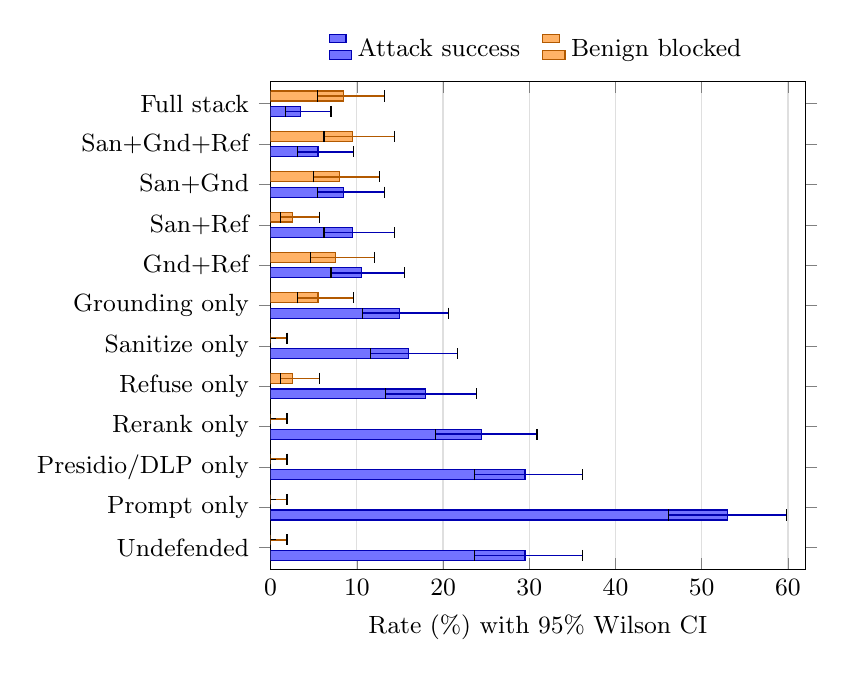
\begin{tikzpicture}
\begin{axis}[
  xbar, scale only axis, width=0.56\columnwidth, height=6.2cm,
  bar width=3.6pt, xmin=0, xmax=62,
  xlabel={Rate (\%) with 95\% Wilson CI}, xlabel style={font=\small},
  symbolic y coords={a0,a1,a2,a3,a4,a5,a6,a7,a8,a9,a10,a11},
  ytick=data, yticklabels={{Full stack},{San+Gnd+Ref},{San+Gnd},{San+Ref},{Gnd+Ref},{Grounding only},{Sanitize only},{Refuse only},{Rerank only},{Presidio/DLP only},{Prompt only},{Undefended}}, y dir=reverse, yticklabel style={font=\small},
  xticklabel style={font=\small}, enlarge y limits=0.05,
  legend style={font=\small, at={(0.5,1.02)}, anchor=south, legend columns=2, draw=none, /tikz/every even column/.append style={column sep=6pt}},
  xmajorgrids, grid style={gray!25},
  error bars/x dir=both, error bars/x explicit,
  error bars/error bar style={line width=0.6pt}]
\addplot[fill=blue!55, draw=blue!70!black] coordinates {
 (3.5,a0) += (3.5,0) -= (1.8,0)
 (5.5,a1) += (4.1,0) -= (2.4,0)
 (8.5,a2) += (4.7,0) -= (3.1,0)
 (9.5,a3) += (4.9,0) -= (3.3,0)
 (10.5,a4) += (5.0,0) -= (3.5,0)
 (15.0,a5) += (5.6,0) -= (4.3,0)
 (16.0,a6) += (5.7,0) -= (4.4,0)
 (18.0,a7) += (5.9,0) -= (4.7,0)
 (24.5,a8) += (6.4,0) -= (5.4,0)
 (29.5,a9) += (6.7,0) -= (5.9,0)
 (53.0,a10) += (6.8,0) -= (6.9,0)
 (29.5,a11) += (6.7,0) -= (5.9,0)};
\addplot[fill=orange!60, draw=orange!70!black] coordinates {
 (8.5,a0) += (4.7,0) -= (3.1,0)
 (9.5,a1) += (4.9,0) -= (3.3,0)
 (8.0,a2) += (4.6,0) -= (3.0,0)
 (2.5,a3) += (3.2,0) -= (1.4,0)
 (7.5,a4) += (4.5,0) -= (2.9,0)
 (5.5,a5) += (4.1,0) -= (2.4,0)
 (0.0,a6) += (1.9,0) -= (0,0)
 (2.5,a7) += (3.2,0) -= (1.4,0)
 (0.0,a8) += (1.9,0) -= (0,0)
 (0.0,a9) += (1.9,0) -= (0,0)
 (0.0,a10) += (1.9,0) -= (0,0)
 (0.0,a11) += (1.9,0) -= (0,0)};
\legend{Attack success,Benign blocked}
\end{axis}
\end{tikzpicture}
\caption{Attack success and benign blocking by configuration, Protocol B ($n=200$ attack and $n=200$ benign rows per arm, current code). San = sanitization, Gnd = grounding gate, Ref = refuse-on-detection.}
\label{fig:asr}
\end{figure}

\begin{figure}[t]
\centering
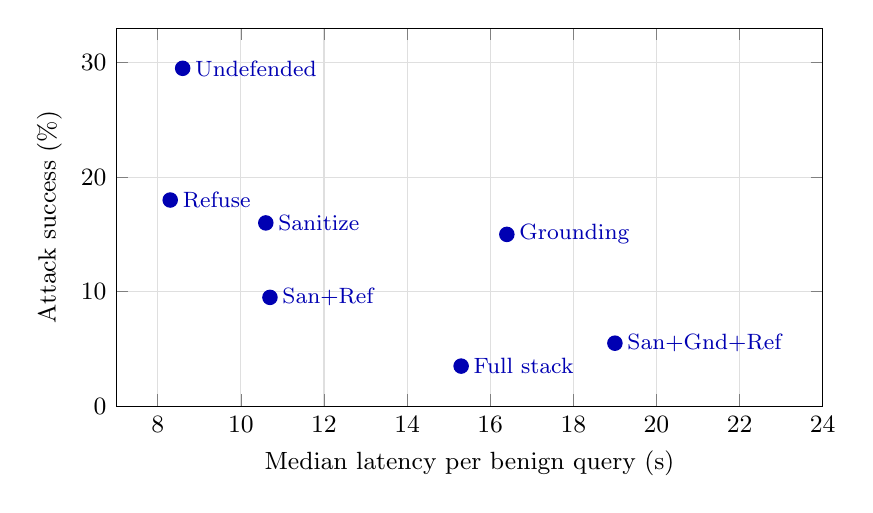
\begin{tikzpicture}
\begin{axis}[
  scale only axis, width=0.74\columnwidth, height=4.8cm,
  xlabel={Median latency per benign query (s)}, ylabel={Attack success (\%)},
  xlabel style={font=\small}, ylabel style={font=\small},
  ticklabel style={font=\small}, xmin=7, xmax=24, ymin=0, ymax=33,
  grid=major, grid style={gray!25},
  nodes near coords, point meta=explicit symbolic,
  every node near coord/.append style={font=\footnotesize, anchor=west, xshift=1pt}]
\addplot[only marks, mark=*, mark size=2.6pt, blue!70!black] coordinates {
 (8.6,29.5)[Undefended]
 (8.3,18.0)[Refuse]
 (10.6,16.0)[Sanitize]
 (16.4,15.0)[Grounding]
 (10.7,9.5)[San+Ref]
 (19.0,5.5)[San+Gnd+Ref]
 (15.3,3.5)[Full stack]};
\end{axis}
\end{tikzpicture}
\caption{Security versus latency (Protocol B, current code). Sanitize+refuse obtains about three quarters of the full-stack ASR reduction (20 of 26 points) for +2\,s; adding grounding obtains most of the remainder for a further 5--8\,s.}
\label{fig:tradeoff}
\end{figure}

\begin{table}[t]
\centering
\caption{Ablation under Protocol B ($n=200$ attack, $n=200$ benign per arm). ASR = attack success rate with Wilson 95\% CI; $p$ = exact McNemar test against the paired undefended arm (``fix/brk'' = discordant rows the configuration fixed / broke). Benign blk = benign rows refused.}
\label{tab:ablation}
\setlength{\tabcolsep}{2.5pt}
\small
\resizebox{\columnwidth}{!}{%
\begin{tabular}{lcccc}
\toprule
Configuration & ASR \% [95\% CI] & fix/brk & $p$ & \makecell{Benign\\blk \%} \\
\midrule
Undefended & 29.5 [23.6, 36.2] & -- & -- & 0.0 \\
\textbf{Full stack (7 layers)} & \textbf{3.5} [1.7, 7.0] & 54/2 & $<\!10^{-13}$ & 8.5 \\
\midrule
\multicolumn{5}{l}{\emph{Leave one out}} \\
\quad $-$ sanitization & 11.0 [7.4, 16.1] & 50/13 & $3\!\times\!10^{-6}$ & 7.5 \\
\quad $-$ grounding gate & 6.5 [3.8, 10.8] & 49/3 & $10^{-11}$ & 2.5 \\
\quad $-$ refuse-on-detection & 6.0 [3.5, 10.2] & 51/4 & $2\!\times\!10^{-11}$ & 7.0 \\
\quad $-$ tightened rerank & 6.0 [3.5, 10.2] & 51/4 & $2\!\times\!10^{-11}$ & 6.5 \\
\quad $-$ guarded prompt & 5.5 [3.1, 9.6] & 53/5 & $3\!\times\!10^{-11}$ & 12.5 \\
\quad $-$ Presidio & 4.0 [2.0, 7.7] & 53/2 & $<\!10^{-13}$ & 8.5 \\
\quad $-$ DLP & 3.5 [1.7, 7.0] & 54/2 & $<\!10^{-13}$ & 8.5 \\
\midrule
\multicolumn{5}{l}{\emph{Single layer only}} \\
\quad Grounding gate & 15.0 [10.7, 20.6] & 29/0 & $4\!\times\!10^{-9}$ & 5.5 \\
\quad Sanitization & 16.0 [11.6, 21.7] & 30/3 & $1.4\!\times\!10^{-6}$ & 0.0 \\
\quad Refuse-on-detection & 18.0 [13.3, 23.9] & 25/2 & $6\!\times\!10^{-6}$ & 2.5 \\
\quad Tightened rerank & 24.5 [19.1, 30.9] & 28/18 & 0.18 & 0.0 \\
\quad Guarded prompt & 53.0 [46.1, 59.8] & 6/53 & $2\!\times\!10^{-10}$ & 0.0 \\
\quad Presidio / DLP & 29.5 [23.6, 36.2] & 0/0 & 1.0 & 0.0 \\
\midrule
\multicolumn{5}{l}{\emph{Subsets}} \\
\quad \textbf{Sanitize+ground+refuse} & \textbf{5.5} [3.1, 9.6] & 48/0 & $7\!\times\!10^{-15}$ & 9.5 \\
\quad Sanitize+ground & 8.5 [5.4, 13.2] & 42/0 & $5\!\times\!10^{-13}$ & 8.0 \\
\quad Sanitize+refuse & 9.5 [6.2, 14.4] & 42/2 & $10^{-10}$ & 2.5 \\
\quad Ground+refuse & 10.5 [7.0, 15.5] & 40/2 & $4\!\times\!10^{-10}$ & 7.5 \\
\bottomrule
\end{tabular}}
\end{table}

\subsection{Comparison with Existing Defenses}
Table~\ref{tab:existing} runs three existing defenses on the same 200 attacks and 200 benign questions, with the same generator and scoring. Spotlighting~\cite{hines2024spotlighting} uses datamarking and regenerates the answers. LLM-Guard~\cite{protectai2024} acts as an input firewall over the query and every passage in the prompt (threshold 0.5). ControlNET~\cite{yao2025controlnet} is reimplemented as described by its authors (Llama-3.1-8B layer-1 activation shift, decision tree) and given exactly the passages the undefended generator received. The two detectors only block or pass, so they are scored on the stored undefended answers of the rows they pass. The full stack outperforms LLM-Guard (3 vs.\ 38 discordant rows, $p=1\times10^{-8}$) and Spotlighting ($p<10^{-9}$) with no significant difference in benign correctness. ControlNET matches the full stack on attack success ($p=0.77$) but answers fewer benign questions correctly (46.0\% vs.\ 52.0\%, $p=0.058$; $p=0.012$ against the three-layer subset). We therefore claim parity with ControlNET, not superiority; its mitigation module is not reimplemented.

\begin{table}[t]
\centering
\caption{Existing defenses on Protocol B: 200 planted attacks and 200 benign questions, same generator and scoring, paired by row. Wilson 95\% CIs; $p$ = exact McNemar test of attack success against the full stack.}
\label{tab:existing}
\setlength{\tabcolsep}{2.5pt}
\small
\resizebox{\columnwidth}{!}{%
\begin{tabular}{lcccc}
\toprule
Defense & ASR \% [95\% CI] & \makecell{Benign\\blocked \%} & \makecell{Benign\\correct \%} & $p$ \\
\midrule
Undefended & 29.5 [23.6, 36.2] & 0.0 & 56.5 & $<\!10^{-13}$ \\
Spotlighting & 23.0 [17.7, 29.3] & 0.0 & 55.5 & $9\!\times\!10^{-10}$ \\
LLM-Guard firewall & 21.0 [15.9, 27.2] & 8.5 & 51.0 & $1\!\times\!10^{-8}$ \\
ControlNET & 4.5 [2.4, 8.3] & 13.5 & 46.0 & 0.77 \\
\midrule
This work, 3 layers & 5.5 [3.1, 9.6] & 9.5 & 52.0 & 0.34 \\
This work, full stack & 3.5 [1.7, 7.0] & 8.5 & 52.0 & -- \\
\bottomrule
\end{tabular}}
\end{table}

\subsection{Conjunctive Detection on Saturated Scores}\label{sec:negative}
Of the 40 conjunctive rows, the gate blocked 6; on the remaining 34 the co-activation detector fired once, and that fire is invalid because both channels were individually above threshold. Recalibration cannot help: class separation is $-0.30$ raw and $-0.39$ calibrated, and a monotone map preserves the overlap. The reason is structural. A valid fire requires the query to pass Stage~3 and the chunk to survive Stage~6, i.e., low injection scores on both channels; a co-activation signal built from those scores is therefore low on exactly the rows it targets, while any payload strong enough to raise it saturates the near-binary classifier and is stopped by Stage~3 or~6 alone. The premise is saturation, which suggests a repair: reading the DeBERTa logit margin as a graded channel gives 24/30 valid fires at 1/80 benign false fires. The repair generalizes poorly: 6/200 false fires on held-out benign questions, 8/30 fires on external BIPIA attacks (4/30 on benign controls), and no context floor separates attack contexts from benign ones. The impossibility is thus specific to saturated channels. It did not cost security here, because Stage~6 redacted every conjunctive chunk.

\subsection{External Benchmarks and the Semantic Gap}\label{sec:external}
On BIPIA, the pipeline blocks 45 of 50 indirect injections (0/50 undefended); of the 5 unblocked, 2 followed the injected instruction. On deepset, the gate flags 17 of 30 real injections at 0/30 benign; on the full test split, letting the gate also flag on the graded margin raises flagged injections from 28/60 to 38/60 at 2/56 benign. Knowledge corruption is different. PoisonedRAG passages are fluent factual text without an instruction signature, Stage~6 redacts none of the 148 injected passages, and ASR is 90.7\% defended vs.\ 91.3\% undefended (7 fixed, 6 broken, $p=1.0$). On our 40-row semantic slice, ASR falls from 75.0\% to 35.0\% ($p=4\times10^{-4}$), but grounding alone has no effect, because a planted fact is ``grounded'' in its passage. An agreement-based generator removes the attack (0/40) only by abstaining (it answers 15 of 40 benign questions), and a routed variant that keeps utility reduces ASR only from 18/40 to 15/40 ($p=0.45$). Table~\ref{tab:external} summarizes the external results. Every effective layer keys on instruction signatures; defending against knowledge corruption requires provenance and corroboration, which this defense class lacks.

\begin{table*}[t]
\centering
\caption{Complete pipeline on independent external sets, paired row by row with an undefended RAG arm on the same rows and poison. ASR = attack's target string in the delivered answer and true answer absent; $p$ = exact McNemar (fixed/broke).}
\label{tab:external}
\setlength{\tabcolsep}{2.5pt}
\small
\begin{tabular}{lrcccc}
\toprule
Set & $n$ & \makecell{Chunk\\redacted} & \makecell{ASR\\undefended} & \makecell{ASR\\defended} & \makecell{fix/brk\\($p$)} \\
\midrule
PoisonedRAG-NQ & 50 & 0/49 & 46 & 44 & 4/2 (0.69) \\
PoisonedRAG-HotpotQA & 50 & 0/50 & 46 & 47 & 1/2 (1.0) \\
PoisonedRAG-MS MARCO & 50 & 0/49 & 45 & 45 & 2/2 (1.0) \\
\textbf{PoisonedRAG, all} & 150 & 0/148 & \makecell{137 (91.3\%)\\{[85.7, 94.9]}} & \makecell{136 (90.7\%)\\{[84.9, 94.4]}} & 7/6 (1.0) \\
\quad same generator$^\ddagger$ & 150 & -- & 137 (91.3\%) & \makecell{128 (85.3\%)\\{[78.8, 90.1]}} & 16/7 (0.09) \\
\midrule
 & & & \multicolumn{2}{c}{Blocked: undef.\ / def.} & \\
BIPIA text attack & 50 & 33/49 & \multicolumn{2}{c}{0/50 / 45/50} & $^\dagger$ \\
\midrule
deepset (gate only) & 30+30 & \multicolumn{4}{l}{Blocked 14/30 (46.7\%), flagged 17/30 (20/30 with graded flag); benign 0/30} \\
\bottomrule
\end{tabular}

\vspace{2pt}{\footnotesize $^\dagger$BIPIA goals are not string-scorable; the 5 unblocked defended rows were read manually: 2 followed the injected instruction, 2 did not, 1 indeterminable. $^\ddagger$Seven-layer harness, \texttt{llama3.2:3b} in both arms; BIPIA 44/50 blocked.\par}
\end{table*}

\textbf{Practical implications.} Any deployment that retrieves from a corpus outsiders can write to (wikis, reviews, tickets, crawled pages) is exposed: one fluent passage that ranks highly for a target question yields confident, citation-backed false answers, and injection classifiers, canaries, and spotlighting are blind to it by design. Deployments should treat retrieval provenance as a security boundary, require corroboration across passages for high-stakes answers, surface citations, and route single-source high-stakes answers to human review.

\subsection{Overhead}\label{sec:overhead}
On benign queries, median latency is 8.6\,s undefended and 15.3\,s for the full stack; the three-layer subset takes 19.0\,s, because it keeps the CPU-bound grounding judge, the dominant cost. Moving the encoders to the GPU in fp16 cuts the full stack's median to 8.6\,s (13.3\,s with CPU encoders in the same session), with identical decisions on all 50 benign questions tested. Peak usage is 6.3\,GB of the 8\,GB GPU and 8.0\,GB of host RAM (Table~\ref{tab:overhead}).

\begin{table}[t]
\centering
\caption{End-to-end latency per query (seconds; median / 95th percentile; 200 rows per cell unless noted) on an RTX 4060 Laptop GPU (8\,GB).}
\label{tab:overhead}
\setlength{\tabcolsep}{3pt}
\small
\resizebox{\columnwidth}{!}{%
\begin{tabular}{lcc}
\toprule
Configuration & Attack rows & Benign rows \\
\midrule
Undefended (single generator) & 9.2 / 13.1 & 8.6 / 12.2 \\
Refuse-on-detection only & 7.5 / 12.2 & 8.3 / 11.6 \\
Sanitize + refuse & 9.7 / 14.9 & 10.7 / 15.1 \\
Sanitize + ground + refuse & 15.9 / 29.2 & 19.0 / 29.5 \\
Full stack, 7 layers (Protocol B) & 15.4 / 24.7 & 15.3 / 21.3 \\
\quad encoders on CPU, rerun ($n=50$) & -- & 13.3 / 20.1 \\
\quad encoders on GPU, fp32 ($n=50$) & -- & 22.6 / 40.7 \\
\quad encoders on GPU, fp16 ($n=50$) & -- & 8.6 / 10.1 \\
\midrule
Full 13 stages, 3-model ensemble & \multicolumn{2}{c}{23.8 (mean, external $n=200$)} \\
ADO baseline~\cite{palleria2026ado} & \multicolumn{2}{c}{31.5 (median, $n=210$)} \\
\bottomrule
\end{tabular}}
\end{table}

\subsection{Threats to Validity}
Components were developed against the Protocol~A slice; Protocol~B, the semantic slice, and the external sets were not used for development. Protocol~B uses one generator, and Ollama GPU generation is not bit-reproducible, which we address with three seeds and a fresh rerun. The knowledge base is small and the generators are 3--7B models; generalization to larger corpora and stronger, adaptive attackers is untested. The ControlNET reimplementation reaches a validation F1 of 0.88 and omits its mitigation module.

\section{Conclusion}
Stage-level attribution of a local defense-in-depth RAG pipeline shows that instruction-carrying attacks are strongly but not completely mitigated (29.5\%$\rightarrow$3.5\% ASR), that three layers carry essentially all of that defense, that the pipeline beats an input firewall and Spotlighting and matches ControlNET on the same attacks, that co-activation detection fails on saturated scores for a provable reason, and that signature-free knowledge corruption remains unmitigated. Practitioners should deploy per-chunk sanitization, grounding, and refusal on detection first, and treat knowledge corruption as requiring provenance controls. Code, data, per-row outputs, and a claim-by-claim checker are available at \url{https://github.com/nahinafrin/multivector-thesis}; an extended version gives all tables and analyses.

\bibliographystyle{IEEEtran}
\bibliography{refs}

\end{document}
